\documentclass{article}

\setlength{\headsep}{0.75 in}
\setlength{\parindent}{0 in}
\setlength{\parskip}{0.1 in}

%=====================================================
% Add PACKAGES Here (You typically would not need to):
%=====================================================

\usepackage[margin=1in]{geometry}
\usepackage{amsmath,amsthm}
\usepackage{fancyhdr}
\usepackage{enumitem}
\usepackage{graphicx}
%=====================================================
% Ignore This Part (But Do NOT Delete It:)
%=====================================================

\theoremstyle{definition}
\newtheorem{problem}{Problem}
\newtheorem*{fun}{Fun with Algorithms}
\newtheorem*{challenge}{Challenge Yourself}
\def\fline{\rule{0.75\linewidth}{0.5pt}}
\newcommand{\finishline}{\vspace{-15pt}\begin{center}\fline\end{center}}
\newtheorem*{solution*}{Solution}
\newenvironment{solution}{\begin{solution*}}{{\finishline} \end{solution*}}
\newcommand{\grade}[1]{\hfill{\textbf{($\mathbf{#1}$ points)}}}
\newcommand{\thisdate}{\today}
\newcommand{\thissemester}{\textbf{Rutgers: Spring 2021}}
\newcommand{\thiscourse}{CS 440: Introduction to Artificial Intelligence} 
\newcommand{\thishomework}{Number} 
\newcommand{\thisname}{Name} 

\newcommand{\thisheading}{
   \noindent
   \begin{center}
   \framebox{
      \vbox{\vspace{2mm}
    \hbox to 6.28in { \textbf{\thiscourse \hfill \thissemester} }
       \vspace{4mm}
       \hbox to 6.28in { {\Large \hfill Project \#\thishomework \hfill} }
       \vspace{2mm}
         \hbox to 6.28in { { \hfill \thisdate \hfill} }
       \vspace{2mm}
       \hbox to 6.28in { \emph{Names: \thisname \hfill }}
      \vspace{2mm}}
      }
   \end{center}
   \bigskip
}

%=====================================================
% Some useful MACROS (you can define your own in the same exact way also)
%=====================================================


\newcommand{\ceil}[1]{{\left\lceil{#1}\right\rceil}}
\newcommand{\floor}[1]{{\left\lfloor{#1}\right\rfloor}}
\newcommand{\prob}[1]{\Pr\paren{#1}}
\newcommand{\expect}[1]{\Exp\bracket{#1}}
\newcommand{\var}[1]{\textnormal{Var}\bracket{#1}}
\newcommand{\set}[1]{\ensuremath{\left\{ #1 \right\}}}
\newcommand{\poly}{\mbox{\rm poly}}


%=====================================================
% Fill Out This Part With Your Own Information:
%=====================================================


\renewcommand{\thishomework}{1: This Maze is on \emph{Fire}} %Homework number
\renewcommand{\thisname}{Aamna Farooq, Nada Elshamaa, and Asma Makhdoom} % Your name
 \graphicspath{ {./images/} }

\begin{document}

\thisheading



\begin{problem}
	Write an algorithm for generating a maze with a given dimension and obstacle density p.
	 
\end{problem}
\begin{solution}
	Please see generateMaze function within generateMaze.py in the code.  
		
%=====================================================
% LaTeX Tip: The figure environment is used for displaying the figure. Inside that, we use \includegraphics for adding a different file for each of the figure.
% What you need to do is to create your figure using any tool you like (including drawing it by hand and scanning it), turn it into a pdf, name it "tree[X].pdf" 
% where you replace [X] by A,B,C, or D depending on which part you are solving (i.e., use treeA.pdf, treeB.pdf,...). Finally, copy the file in the same directory
% as this template and you should see that getting compiled into your solution. You can change the width=0.5\textwidth command to fix the size of the figure
% in the final PDF. Finally, if the figure appears in the next page, do not worry about it as they will still have the proper caption. 
%=====================================================		
\end{solution}
\smallskip

\begin{problem}
	Write a $DFS$ algorithm that takes a maze and two locations within it, and determines whether one is reachable from the other. Why is $DFS$ a better choice than $BFS$ here? For as large a dimension as your system can handle, generate a plot of 'obstacle density p' vs 'probability that S can be reached from G'
	
\end{problem}

\smallskip

\begin{solution} \hfill \\
	If you want an algorithm that takes a maze and two locations within it, and determine whether one is reachable from the other $DFS$ is a better choice than $BFS$ because in this algorithm the optimal path does not matter. The purpose of $BFS$ is to find an optimal path but since we don't care about that we should choose the algorithm that uses less compute power, which is $DFS$.
	
	\begin{figure}[h]
	\centering
	\IfFileExists{images/p2.png}{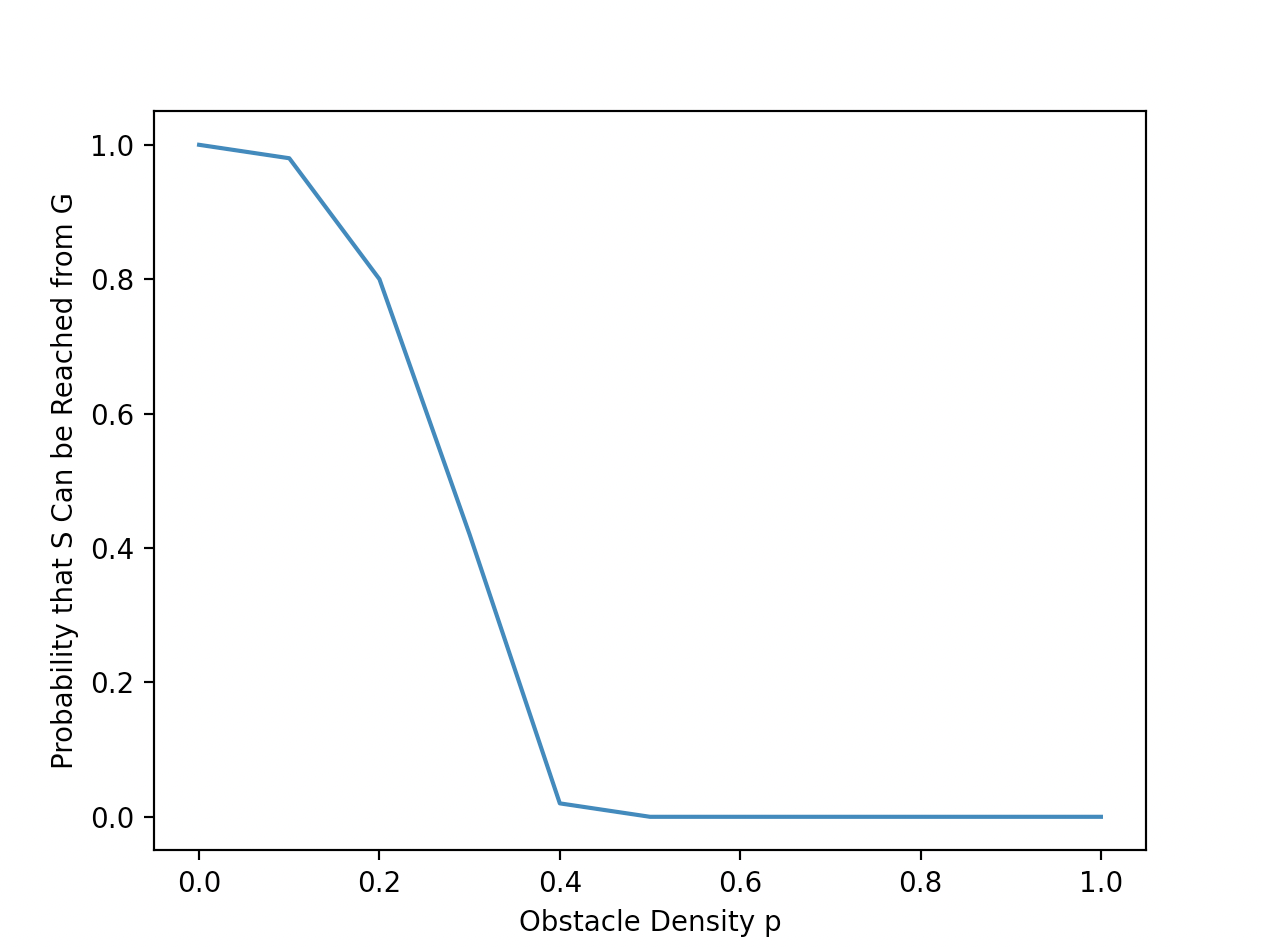
\includegraphics[width=0.7\textwidth]{images/p2.png}}{No Figure Yet}
% 	\includegraphics[width=12cm]{dim100,50avg,step01}
	\caption{Plot using a dimension of 100, average of 50, 0$<$p$<$1 with step = 0.1}
	\end{figure}
	
\end{solution}


\smallskip


\begin{problem}
	Write $BFS$ and $A*$ algorithms (using the euclidean distance metric) that take a maze and determine the shortest path from $S$ to $G$ if one exists. For as large a dimension as your system can handle, generate a plot of the average $'number$ $of$ $nodes$ $explored$ $by$ $BFS$ - $number$ $of$ $nodes$ $explored$ $by$ $A*$' vs $'obstacle$ $density$ $p'$. If there is no path from $S$ to $G$, what should this difference be? 
	
\end{problem}

\smallskip

\begin{solution}
    If there was no path from S to G then there would be no difference between the number of nodes explored. This is because A* and BFS each would try to exhaust every possible option and would therefore have the same number of nodes explored.
    
	\begin{figure}[h]
	\centering
	\IfFileExists{images/dim100,50avg,step01.png}{\includegraphics[width=0.7\textwidth]{images/dim100,50avg,step01.png}}{No Figure Yet}
% 	\includegraphics[width=12cm]{dim100,50avg,step01}
	\caption{Plot using a dimension of 1000, average of 50, 0$<$p$<$1 with step = 0.01}
	\end{figure}
	
\end{solution}

\smallskip

\begin{problem}
	What's the largest dimension you can solve using $DFS$ at p = 0.3 in $less$ than a minute? What's the largest dimension you can solve using $BFS$ at p = 0.3 in $less$ than a minute? What's the largest dimension you can solve using $A*$ at p = 0:3 in $less$ than a minute?  
\end{problem}

\smallskip

\begin{solution}
	Solution to problem four goes here. 
\end{solution}

\smallskip

\begin{problem}
	Describe your improved Strategy 3. How does it account for the unknown future?
\end{problem}

\smallskip

\begin{solution}
	Our Strategy 3 algorithm tries to account for unknown future by trying to predict the path of the fire. We do this in 2 ways. 
    \\\\
	1. We employ a deterministic approach where we assume the fire will spread 100\% of the time to all nodes it could possibly spread to for each time step. Based on this we generate a 3-D maze which has a maze for each time step. The size of the 3-D maze is dependent on the distance from the current position to the fire which is calculated using Manhattan distance. Based on the number of time steps we traverse through the 3-D maze and try to get as far as we can with a deterministic approach. 
	\\
	If this deterministic approach is unable to reach the goal, we use 2. 
	\\\\
	2. We employ a probabilistic approach where we assume where the fire will spread by generating an average of 10 possible mazes for each time step with the actual value of q. The average maze holds a probability for each cell catching on fire. Using each resulting average maze we generate a 3-D maze that holds an average maze for each time step, the number of time steps depending upon the distance of the current position on the path from the fire. From the last position of the path we traverse through the maze, choosing the cell that has the least probability of catching on fire at each time step.
	\\ 
	Once we have traversed the length of the time steps calculated using the distance from the fire, if we have not reached the goal we revert to the deterministic approach once again.
	\\\\
	Our strategy 3 is done using $A*$. $A*$ typically uses a heuristic value that is derived from calculating the euclidean distance of the current position from the goal and adding that to the traversed distance. This value is appended to a priority queue, where values are then chosen and dequeued based on their priority (smaller distances have higher priority). We altered this algorithm for strategy 3 by instead including a priority value that consisted of a tuple of 2 values. Our first value in the tuple consisted of the probability of that cell catching on fire, as calculated in our 3-D maze, summed with the probability of fire on that path so far. The second value in the tuple was of the distance heuristic (euclidean) that is typically used in $A*$. This tuple sorts the queue in ascending based on the first value and sub-sorts in ascending order based on the second value. We employed the use of a tuple in our priority queue because we wanted to prioritize survivability over getting the shortest possible path. 
	\\\\
	To optimize our algorithm and to preserve compute power we performed a $DFS$ algorithm on our initial maze before the fire has spread (time step = 0) to ensure that finish is reachable from start initially. Otherwise, it returns the maze because there is no possible path to finish.
	
\end{solution}

\smallskip

\begin{problem}
	Plot, for Strategy 1, 2, and 3, a graph of `average strategy success rate' vs `flammability q' at p = 0.3. Where do the different strategies perform the same? Where do they perform differently? Why?
\end{problem}

\smallskip

\begin{solution} \hfill \\
    \begin{figure}[h]
	\centering
	\IfFileExists{images/P6ST1.png}{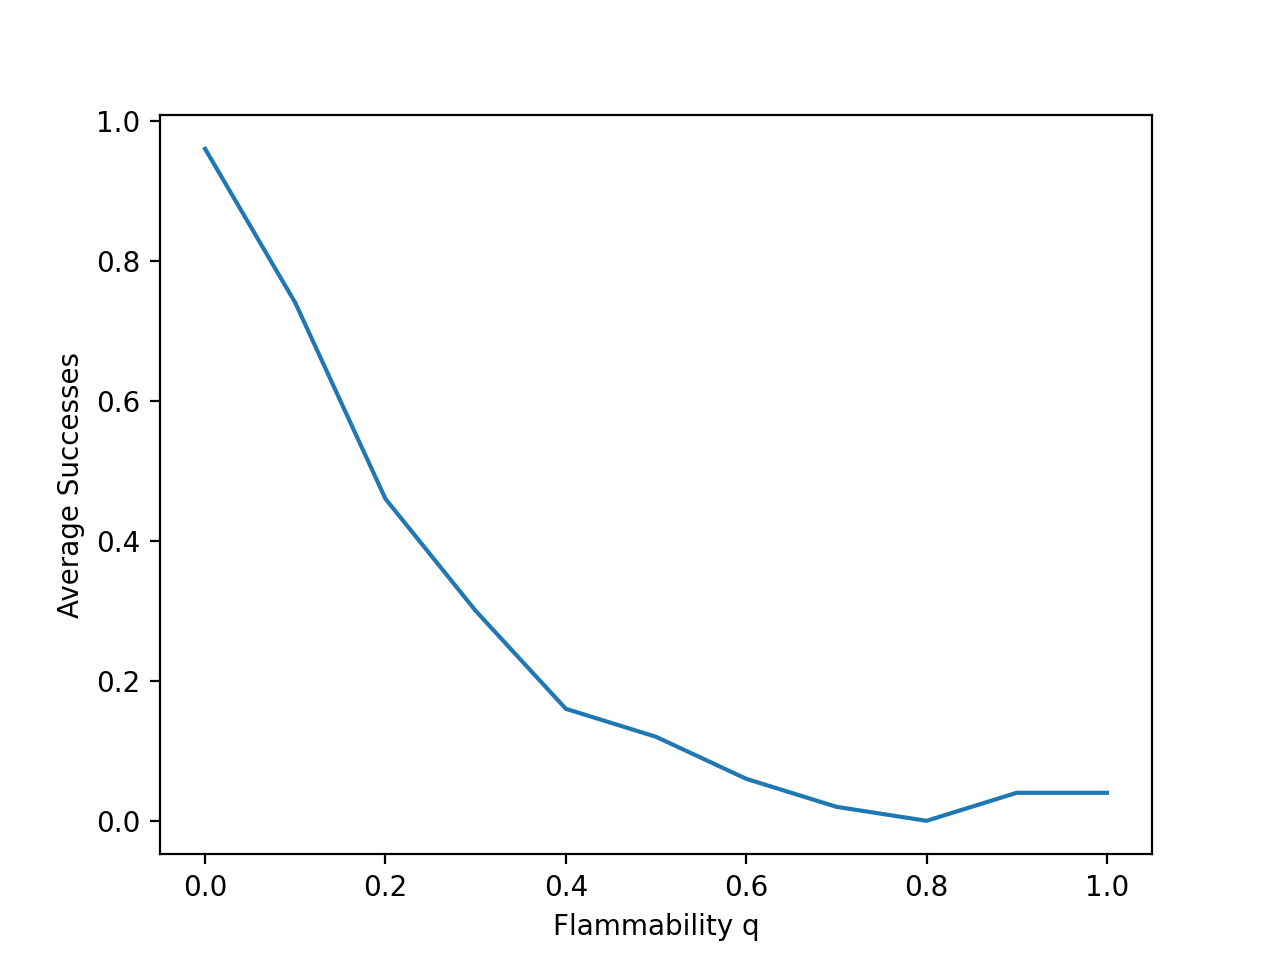
\includegraphics[width=0.7\textwidth]{images/P6ST1.png}}{No Figure Yet}
% 	\includegraphics[width=12cm]{dim100,50avg,step01}
	\caption{Strategy 1, Using a dimension of 100, average of 50, p=0.3, q with step of 0.1.} 
	\vspace{1cm}
	\end{figure} 
    
    \begin{figure}[h]
	\centering
	\IfFileExists{images/P6ST2.png}{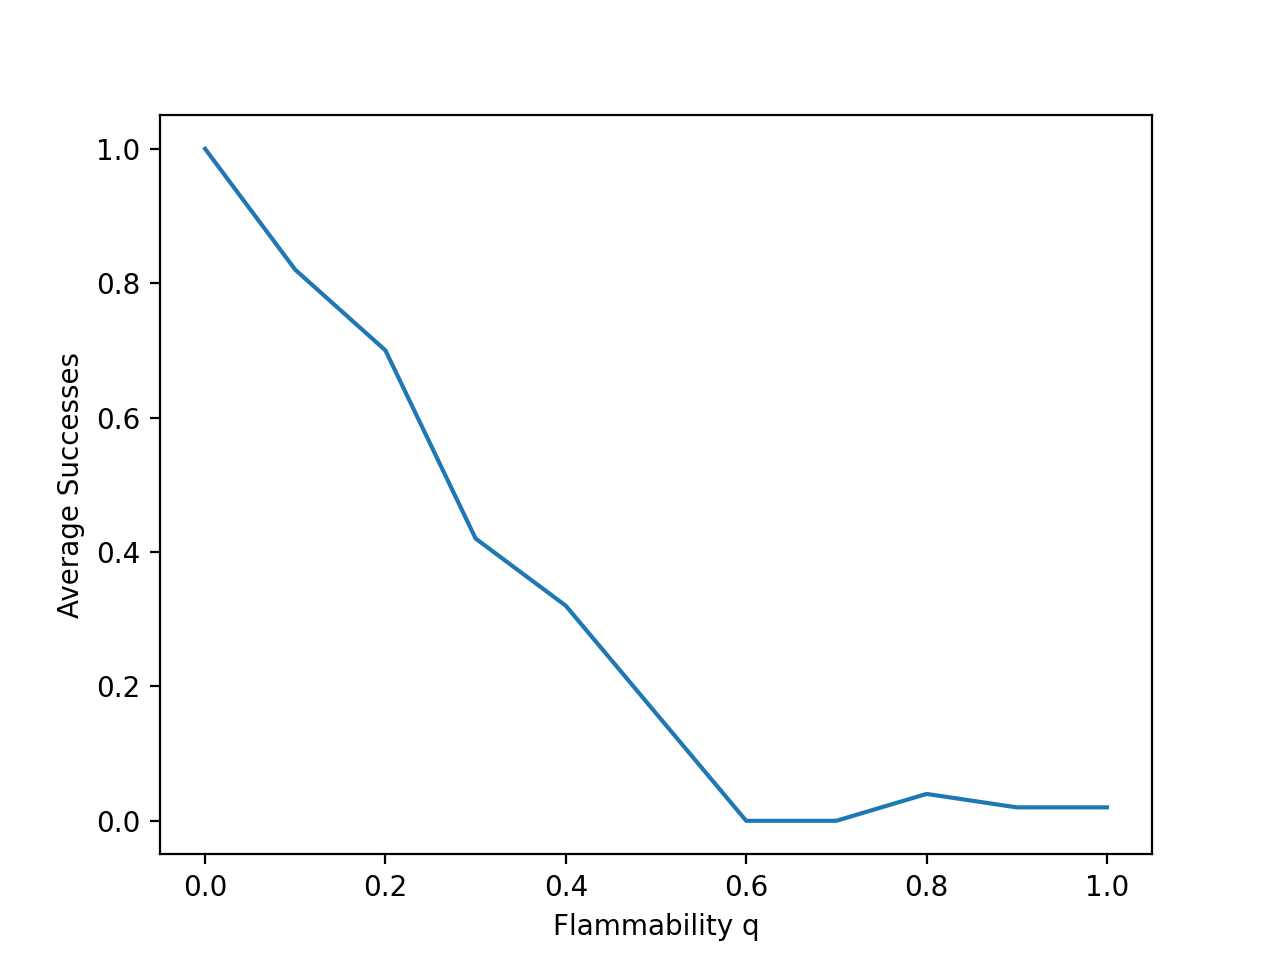
\includegraphics[width=0.7\textwidth]{images/P6ST2.png}}{No Figure Yet}
% 	\includegraphics[width=12cm]{dim100,50avg,step01}
	\caption{Strategy 2, Using a dimension of 100, average of 50, p=0.3, q with step of 0.1.}
	\end{figure}
    
    \begin{figure}[h]
	\centering
	\IfFileExists{images/P6ST3.png}{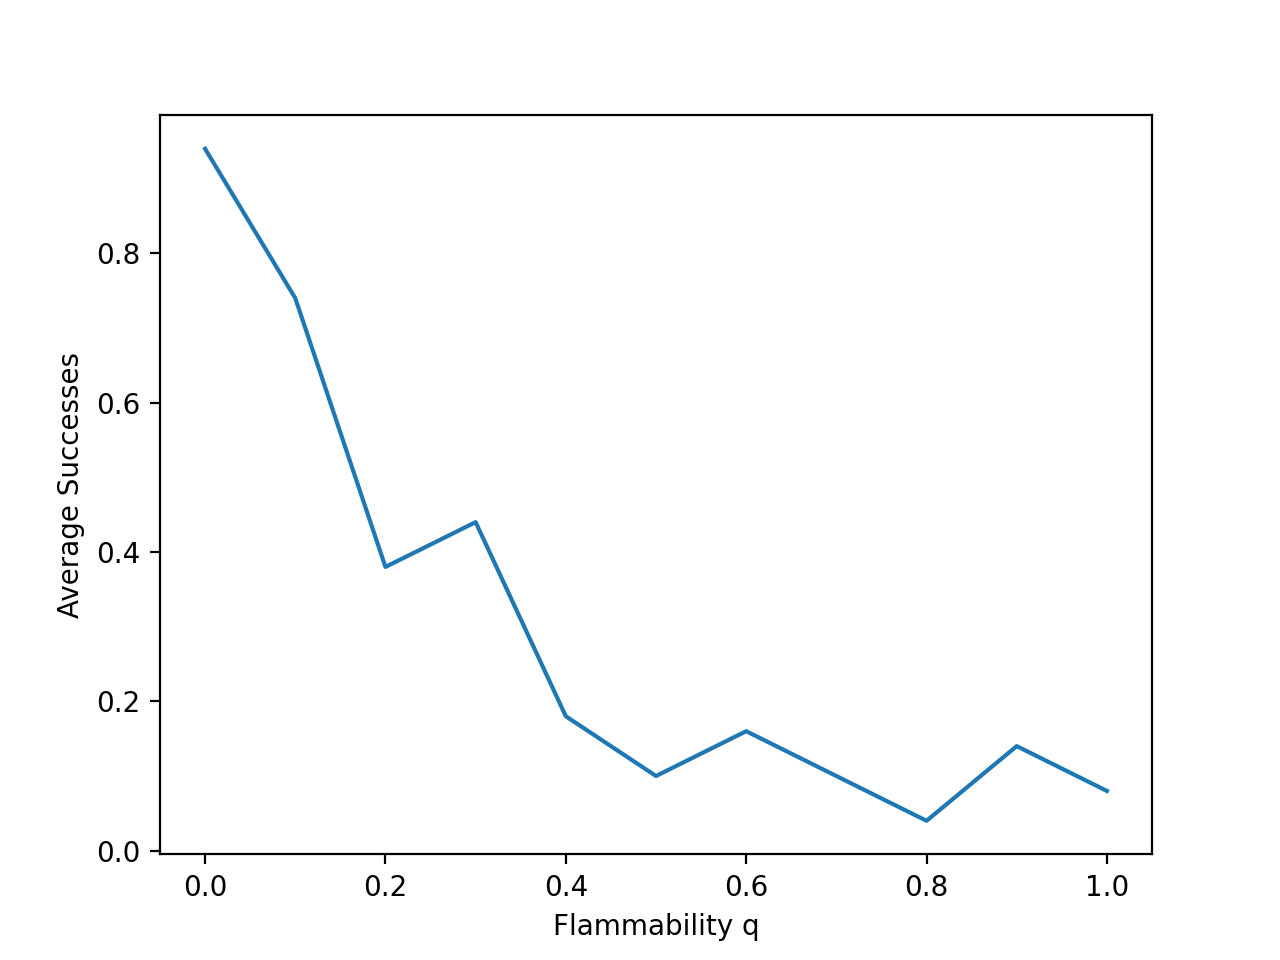
\includegraphics[width=0.7\textwidth]{images/P6ST3.png}}{No Figure Yet}
% 	\includegraphics[width=12cm]{dim100,50avg,step01}
	\caption{Strategy 3, Using a dimension of 10, average of 50, p=0.3, q with step of 0.1.}
	\end{figure}
    
\end{solution}

\smallskip

\begin{problem}
	If you had unlimited computational resources at your disposal, how could you improve on Strategy 3? 
\end{problem}

\smallskip

\begin{solution} \hfill \\
	If we had unlimited computational resources we wouldn't need to rely on a deterministic approach to get a path. The purpose of our deterministic approach was to find a path from start to finish in less time because if there exists a path when q=1, that path exists for all other values of q. Using the deterministic approach in our algorithm reduces our computational power because using this approach does not require calculating an average of mazes. Therefore, we would completely rely on the probabilistic approach in order to find the path from start to finish. The probabilistic approach is a more accurate representation of the maze because it uses the real value of q instead of q=1 in order to sample what the fire looks like in future time steps. \\ \\
	Another approach we could take if we had unlimited computational resources is to calculate the state of the fire as far into the future as possible (i.e. until the goal can be reached). In our current algorithm, we calculate the number of time steps to look ahead in the future by how far we are from the fire currently. This caps how far we look into the future but if we had unlimited computational resources we would not need to place a limit on the number of steps to look ahead. \\ \\
    Lastly, we would want to increase the number of samples we use to average each probability maze for each time step. Currently, we are only sampling 10 mazes for each time step. By gathering more samples, we will have a more accurate picture of what the fire could look like at that time step. \\
\end{solution}

\smallskip

\begin{problem}
	If you could only take ten seconds between moves (rather than doing as much computation as you like), how would that change your strategy? Describe such a potential Strategy 4.
\end{problem}

\smallskip

\begin{solution} \hfill \\
	 
\end{solution}

\smallskip

\end{document}